\chapter{Reti Logiche e Combinatorie} 

\section{Alcuni componenti standard}

Le tabelle di verità che vediamo si convertono in reti logiche. Una tabella di verità con $ n $ ingressi ha $ 2^n $ righe e corrisponde ad un componente logico di un circuito con $ n $ input. Vediamo alcuni oggetti utili. Ricordiamo che i passaggi per definire un componente in forma di rete logica sono: 

\begin{enumerate}
	\item Definizione della funzione con tabella di verità
	\item Conversione della funzione normalizzata in somma di prodotti
	\item Conversione a circuito con porte AND/OR/NOT
\end{enumerate}

\paragraph{Multiplexer (k commutatore)}
Un multiplexer o commutatore è un circuito, ad esempio, con due 2 ingressi, con un ingresso aggiuntivo chiamato di \textit{controllo} che permette di alternare quale sarà l'input che verrà copiato in output.

\begin{figure}[H]
	\centering
	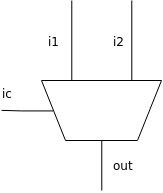
\includegraphics[]{2x1mux-gate}
	\caption{Multiplexer 2 vie 1 bit}
\end{figure}

\begin{table}[H]
	\centering
	\caption{Tabella di verità di un multiplexer a due vie da un bit}
	\label{tab:multiplexer1}
	\begin{tabular}{|lll|l|}
		\hline
		ictrl & $ in_1 $ & $ in_2 $ & out \\ \hline
		0     & 0   & 0   & 0   \\
		0     & 0   & 1   & 0   \\
		0     & 1   & 0   & 1   \\
		0     & 1   & 1   & 1   \\ \hline
		1     & 0   & 0   & 0   \\
		1     & 0   & 1   & 1   \\
		1     & 1   & 0   & 0   \\
		1     & 1   & 1   & 1   \\ \hline
	\end{tabular}
\end{table}

\begin{figure}[H]
	\centering
	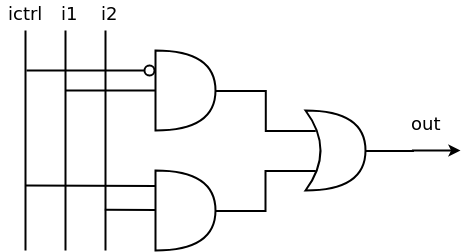
\includegraphics[width=0.68\textwidth]{2x1mux}
	\caption{Circuito logico di un Multiplexer 2 vie 1 bit}
\end{figure}



La funzione è definita come $ out = \overbar{ic} \cdot in_1 \cdot \overbar{in_2} + \overbar{ic} \cdot in_1 \cdot in_2 + ic \cdot \overbar{in_1} \cdot in_2 + ic \cdot in \cdot in_2 $ e si può ridurre in $ out = \overbar{ic} \cdot in_1 + ic \cdot in_2 $. Le tabelle di verità semplificate ci permettono di dedurre direttamente la formula ridotta. Ad esempio, la tabella seguente corrisponde a quella antecedente.
\begin{table}[H]
	\centering
	\caption{Tabella di verità semplificata di un multiplexer a due vie da un bit}
	\label{tab:multiplexer2}
	\begin{tabular}{|lll|l|}
		\hline
		ictrl & in1 & in2 & out \\ \hline
		0     & 0   & -   & 0   \\
		0     & 1   & -   & 1   \\ \hline
		1     & -   & 0   & 0   \\
		1     & -   & 1   & 1   \\ \hline
	\end{tabular}
\end{table}

\paragraph{Multiplexer a 4 Input}
Un multiplexer a 4 input ha bisogno di due bit di controllo. Avendo 6 ingressi, con porte da 8 ingressi massimo $ \implies \ceil*{ log_8(6)} $ livelli di porte.


\begin{figure}[H]
	\centering
	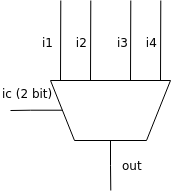
\includegraphics[]{4x1mux-gate}
	\caption{Multiplexer 4 vie 1 bit}
\end{figure}

\begin{table}[H]
	\centering
	\caption{Tabella di verità semplificata di un multiplexer a quattro vie da un bit}
	\label{tab:multiplexer3}
	\begin{tabular}{|llllll|l|}
		\hline
		$ ic_1 $ & $ ic_2 $ & $ in_1 $ & $ in_2 $ & $ in_3 $ & $ in_4 $ & out \\ \hline
		0     & 0     & 1     & -     & -     & -     & 1   \\ \hline
		0     & 1     & -     & 1     & -     & -     & 1   \\ \hline
		1     & 0     & -     & -     & 1     & -     & 1   \\ \hline
		1     & 1     & -     & -     & -     & 1     & 1   \\ \hline
	\end{tabular}
\end{table}


La formula di verità corrispondente sarà
\[ \text{out} = (\overbar{ic_1} \cdot \overbar{ic_2} \cdot in_1) + (\overbar{ic_1} \cdot ic_2 \cdot in_2) + (ic_1 \cdot \overbar{ic_2} \cdot in_3) + (ic_1\cdot ic_2 \cdot in_4)  \]

I livelli delle porte AND saranno $ log_8(n+1) $

\begin{figure}[H]
	\centering
	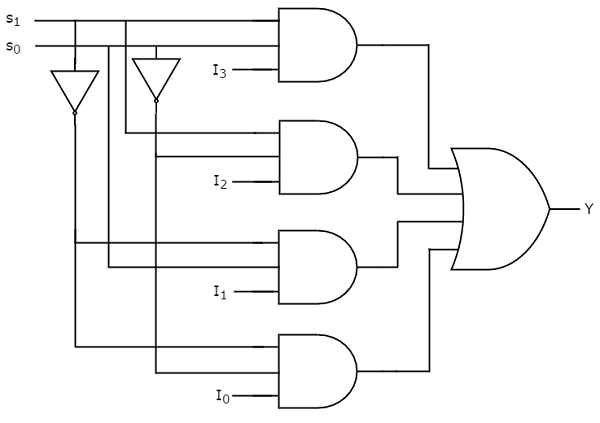
\includegraphics[width=0.75\textwidth]{4x1mux}
	\caption{Circuito logico di un Multiplexer 4 vie 1 bit}
\end{figure}

\paragraph{Commutatori (multiplexer) composti}
Un commutatore multiplo da 1 bit con un numero di vie $ y $, con $ y = 2^x \land x \in \N $ e $ y > 2 $ si può costruire a partire da un albero con $ log_2y $ livelli di multiplexer da 2 vie a 1 bit. Dove ogni bit di controllo del multiplexer complessivo controlla un livello singolo dell'albero.

\centerfig{0.75}{4x1mux-multiple}{Multiplexer 4 vie 1 bit composto da due Multiplexer 2x1}

\paragraph{Multiplexer a 2 vie da k bit}

Un commutatore a 2 vie da $ k $ bit si costruisce con $ k $ commutatori a 2 vie ad 1 bit. Dove ogni commutatore 2x1 accetta in input le corrispettive vie di ogni bit, gli output saranno i $ k $ bit corrispondenti ad ogni Multiplexer.

\diagram{2x4mux.tex}{Multiplexer 2 vie da 4 bit}


\paragraph{Sommatore di numeri}
Un sommatore è un componente che somma due numeri in input e restituisce in output un risultato ed un riporto.

\begin{table}[H]
	\centering
	\caption{Tabella di verità di una somma di due numeri da un bit.}
	\label{tab:sum1bit}
	\begin{tabular}{|lll|l|l|}
		\hline
		$ x_{1} $ & $ x _{2} $ & $ r_0 $ & $ z_1 $ & $r_1$ \\ \hline
		0         & 0          & 0       & 0       & 0     \\
		0         & 0          & 1       & 1       & 0     \\
		0         & 1          & 0       & 1       & 0     \\
		0         & 1          & 1       & 1       & 0     \\
		1         & 0          & 0       & 1       & 0     \\
		1         & 1          & 0       & 0       & 1     \\
		1         & 0          & 1       & 0       & 1     \\
		1         & 1          & 1       & 1       & 1     \\ \hline
	\end{tabular}
\end{table}

\diagram{sum.tex}{Sommatori di due numeri}

Analogamente ai commutatori si possono costruire sommatori di 2 numeri a più bit a partire da sommatori di 2 numeri da 1 bit.


\paragraph{Esercizio}
Realizzare la tabella di verità e circuito di un demultiplexer a 2 vie da 1 bit.

\paragraph{Encoder}
Un encoder è un circuito che converte $ 2^n $ linee in input in un codice di $ n $ bit. 

\begin{table}[H]
	\centering
	\caption{Tabella di verità di encoder da 2 bit.}
	\label{tab:2bitencoder}
	\begin{tabular}{|llll|ll|}
		\hline
		a & b & c & d & z & t \\ \hline
		0 & 0 & 0 & 1 & 0 & 0 \\
		0 & 0 & 1 & 0 & 0 & 1 \\
		0 & 1 & 0 & 0 & 1 & 0 \\
		1 & 0 & 0 & 0 & 1 & 1 \\ \hline
	\end{tabular}
\end{table}

\diagram{4x2encoder.tex}{Encoder di un numero da 2 bit.}

Gli output dell'encoder a 2 bit saranno
\[ z = \overbar{a}b\overbar{cd}+a\overbar{bcd} = \overbar{cd}(\overbar{a}b+a\overbar{b}) \]
\[ t = \overbar{ab}c\overbar{d}+a\overbar{bcd} \]


\paragraph{Decoder}
Un decoder esegue l'operazione opposta.

\begin{table}[H]
	\centering
	\caption{Tabella di verità di un decoder da 2 bit.}
	\label{tab:2bitdecoder}
	\begin{tabular}{|ll|llll|}
		\hline
		a & b & u & v & z & t \\ \hline
		0 & 0 & 0 & 0 & 0 & 1 \\
		0 & 1 & 0 & 0 & 1 & 0 \\
		1 & 0 & 0 & 1 & 0 & 0 \\
		1 & 1 & 1 & 0 & 0 & 0 \\ \hline
	\end{tabular}
\end{table}

Gli output saranno $ u = ab, v = a\overbar{b}, z = \overbar{a}b, t = \overbar{ab} $

\diagram{4x2decoder.tex}{Decoder di un numero da 2 bit.}


\paragraph{Confrontatore}
Un confrontatore (comparatore) confronta due configurazioni di bit e controlla che siano uguali. Un confrontatore da 1 bit è esattamente un gate NOT XOR.

\[ z = ab + \overbar{ab} \]

\begin{table}[H]
	\centering
	\caption{Tabella di verità di un confrontatore da 1 bit.}
	\label{tab:2bitcomparator}
	\begin{tabular}{|ll|l|}
		\hline
		a & b & t \\ \hline
		0 & 0 & 1 \\
		0 & 1 & 0 \\
		1 & 0 & 0 \\
		1 & 1 & 1 \\ \hline
	\end{tabular}
\end{table}

\diagram{confrontatore.tex}{Confrontatore da 1 bit}

Per realizzare un confrontatore da più bit si mettono in parallelo più confrontatori da un solo bit e si uniscono gli output con un albero di AND.

Un confrontatore a 2 bit impiegherà tempo $ 2\Delta t + \Delta t $

Per confrontare valori da $ n $ bit si impiegherà però un tempo di $ \ceil{\log_kn}(\Delta t \cdot \text{ ogni livello AND})$

\paragraph{Confronto maggiore}
In maniera simile ad un confrontatore si può realizzare un componente che controlla se un numero di $ n $ bit è maggiore di un altro.

\begin{table}[H]
	\centering
	\caption{Tabella di verità di un confronto maggiore da 2 bit.}
	\label{tab:2bitgreater}
	\begin{tabular}{|ll|ll|l|}
		\hline
		$ x_0 $ & $ x_1 $ & $ y_0 $ & $ y_1 $ & z \\ \hline
		0       & 0       & -       & -       & 0 \\
		0       & 1       & 0       & 0       & 1 \\
		1       & -       & 0       & -       & 1 \\
		1       & 1       & -       & 0       & 1 \\ \hline
	\end{tabular}
\end{table}

% Please add the following required packages to your document preamble:
% \usepackage[table,xcdraw]{xcolor}
% If you use beamer only pass "xcolor=table" option, i.e. \documentclass[xcolor=table]{beamer}
\begin{table}[H]
	\centering
	\caption{Mappa di Karnaugh di un confrontatore dell'operatore maggiore da 2 bit.}
	\label{tab:2bitgreater}
	\begin{tabular}{|l|llll|}
		\hline
		$ y_1y_0 \backslash x_1x_0 $ & 00 & 01 & 11                        & 10                        \\ \hline
		00                         & 0  & 1  & \cellcolor[HTML]{FFCCC9}1 & \cellcolor[HTML]{FFCCC9}1 \\
		01                         & 0  & 0  & \cellcolor[HTML]{FFCCC9}1 & \cellcolor[HTML]{FFCCC9}1 \\
		11                         & 0  & 0  & 0                         & 0                         \\
		10                         & 0  & 0  & 1                         & 0                         \\ \hline
	\end{tabular}
\end{table}

La formula booleana ottenuta è $ z = x_0\overbar{y_1y_0} + x_1\overbar{y_1} + x_1x_0\overbar{y_0} $

\paragraph{ALU}
Una ALU, ovvero Arithmetic Logic Unit è un componente che in genere, in input accetta due parole $ x,y $ entrambe da $ n $ bit, e può fare due o più operazioni. L'operazione viene selezionata attraverso uno o più bit di controllo. In output ci sarà un uscita da $ n $ bit. Ad esempio, prendiamo una ALU a 4 bit con somma/sottrazione, che accetterà un solo bit di controllo.

\centerfig{0.5}{alusymbol}{Simbolo di una ALU}

I livelli di porte AND saranno $ \ceil{\log_k8} $ che verrano sommati ai livelli di porte OR che saranno $ \log_k(128) $. Le ALU si distinguono fra intere e a floating point. Per semplicità vedremo le ALU intere con somma e moltiplicazione.

\centerfig{1}{74181aluschematic}{Schematica del circuito integrato della ALU \href{https://en.wikipedia.org/wiki/74181}{74181}, la prima ALU completa su un singolo chip.}


\paragraph{Multiply and Add}
Un componente Multiply and Add (MUL\&ADD) è un componente ALU che realizza l'operazione matematica $ \sum_{i}x_iy_i $, ovvero prende gli ingressi $ x_i,y_i $, li moltiplica e li accumula sommando.

% TODO immagine MULADD

\paragraph{Ritardi di propagazione}

Sappiamo che il cambiamento fra HIGH e LOW (0 e 1) nei circuiti digitali non è istantaneo. A volte, il ritardo di propagazione dei transistor può causare dei glitch (fluttuazioni) che potrebbero causare una lettura incorretta dell'output di un circuito. Per ovviare a questo problema si introduce un componente chiamato \textbf{clock}, che scandisce un ciclo preciso per permettere ai valori di propagarsi nei circuiti e leggere l'output preciso alla fine della propagazione $ \Delta t $.

% TODO disegno da quaderno delay transistor e glitch


\section{Reti sequenziali e Automi}

Abbiamo visto nel corso di programmazione 1 gli automi a stati finiti (Finite State Machines o FSM). Per ora, abbiamo visto circuiti logici che implementano funzioni senza stato. Per implementare lo stato possiamo utilizzare gli automi a stati finiti. In un automa di Moore gli output sono determinati solo dallo stato corrente, mentre negli automi di Mealy gli output sono determinati sia dallo stato corrente che dagli input correnti.

\centerfig{0.75}{moore_mealy}{Automi di Moore e Automi di Mealy}

Per portare un Automa di Mealy ad una rete sequenziale abbiamo bisogno di tre blocchi di una rete combinatoria. Uno che dallo stato precedente $ s $ e dall'input $ x $ dia in output l'uscita $ z $, e un altro che ricevendo $ x,s $ in input restituisca $ s^1 $ (lo stato del prossimo nodo del grafo) e un \textbf{SR Latch} (o \textbf{flip-flop}). I flip-flop possono essere di tipo $ SR, D, T $ e $ JK $.
 
% TODO disegno rete combinatoria di un automa

\paragraph{SR Latch o Flip Flop}

Un componente SR Latch è un componente che implementa un bit di memoria. Impostando l'input $ S=1 $ (bit di set) e $ R=0 $  (bit di reset) l'output sarà $ Q=1,\overbar{Q}=0 $ mentre impostando gli input $ S=0,R=1 $ l'output è $ Q=0,\overbar{Q}=1 $. Il fulcro della funzionalità di un SR Latch è che se entrambi gli input $ S=0,R=0 $ allora l'output è in uno stato detto \textbf{latch}, ovvero che "ricorda" lo stato precedente.

\centerfig{0.75}{srlatch}{Tabella di Verità e circuito di un SR Latch}

\paragraph{Clock e D-latch}

Introduciamo un componente fondamentale, il \textbf{clock}, che introduce una dimensione temporale nelle reti combinatorie scandendo un \textbf{ciclo}. Un ciclo di clock ha lunghezza $ \tau $. Possiamo così estendere un SR Latch rendendolo un \textbf{D-Latch}, che riceve in input soltanto il ciclo di clock e un bit $ D $, ovvero il bit che va "ricordato". Per evitare \textbf{glitch} possiamo scrivere sul D-Latch soltanto quando il segnale di clock è nello stato HIGH.

\centerfig{0.75}{dlatch}{Un componente D-latch}
\centerfig{0.75}{dlatch_timing}{Diagramma temporale di un D-latch}

\subsection{Realizzazione di una rete sequenziale di un Automa di Mealy con un clock e registri}
Consideriamo, ad esempio, un automa che calcola la parità del numero di $ 1 $ in una sequenza di bit. Ricevendo in input una sequenza di bit $1, 0, 0, 0, 1, 0, 1 $ ad esempio restituirebbe in output $ 0, 1, 1, 1, 1, 0, 0 $ (l'output diventa high)

\begin{figure}[H]
	\centering
	\caption{Automa di parità di una sequenza di bit}
	\begin{tikzpicture}[->,>=stealth',shorten >=1pt,auto,node distance=3.5cm]
	
	\node[state,accepting] (A)                    {$q_a$};
	\node[state]         (B) [right of=A] {$q_b$};
	
	\path 	(A)		edge [bend left]  	node {$\dfrac{x=1}{z=0}$} (B)
	edge [loop above] 	node {$\dfrac{x=0}{z=1}$} (A)
	(B) 	edge [loop above] 	node {$ \dfrac{x=1}{z=1} $} (B)
	edge [bend left] 	node {$ \dfrac{x=1}{z=1} $} (A);
	\end{tikzpicture}
\end{figure}


Per trasformare l'automa di Mealy in una rete sequenziale avremo una rete combinatoria che calcola lo stato successivo, un registro che mantiene lo stato e una rete combinatoria che calcola l'uscita. Siccome l'automa di Mealy usa l'input $ x $ per decidere le transizioni, l'input $ x $ dovrà essere passato ad entrambe le reti combinatorie dei nodi del grafo.

Chiamiamo la prima rete combinatoria $ \sigma $ e la seconda $ \omega $

\begin{table}[H]
	\centering
	\caption{Tabella di verità della rete combinatoria $ \sigma $}
	\label{tab:mealysigma1}
	\begin{tabular}{|ll|l|}
		\hline
		x & s & s' \\ \hline
		0 & 0 & 0  \\
		1 & 0 & 1  \\
		0 & 1 & 1  \\
		1 & 1 & 0  \\ \hline
	\end{tabular}
\end{table}

\begin{table}[H]
	\centering
	\caption{Tabella di verità della rete combinatoria $ \omega $}
	\label{tab:mealyomega1}
	\begin{tabular}{|ll|l|}
		\hline
		x & s & z \\ \hline
		0 & 0 & 1 \\
		1 & 0 & 0 \\
		0 & 1 & 0 \\
		1 & 1 & 1 \\ \hline
	\end{tabular}
\end{table}

\diagram{mealyautomata1.tex}{Rete sequenziale dell'automa di Mealy in figura precedente}

